\documentclass[12pt, a4paper]{article} % свойства докуменат
\usepackage[utf8]{inputenc} % хотим нормальную кодировку
\usepackage[T2A]{fontenc} % тип шрифта, по-моему
\usepackage[russian]{babel} % русские буквы и обозначения
\usepackage{graphicx, xcolor} % графика
\usepackage{subfiles} % царская разбивка на много файлов
\usepackage{amsmath} % различные нужные символы, типа \geqslant
\usepackage{amssymb} % еще немного символов
\usepackage{import} % для включения рисунков
\usepackage{xifthen}
\usepackage{pdfpages}
\usepackage{transparent}
\usepackage{titlesec} % для настройки заголовков и секций вообще
\usepackage{caption} % для подписей к рисункам на 2 строки
\usepackage[outdir=./figures/]{epstopdf}
\usepackage{multicol}
\usepackage{float}
\usepackage{mathrsfs}

% комманда для царского добавления в документ векторной графики
\newcommand{\incfig}[1]{%
    \def\svgwidth{\columnwidth}
    \import{figures/}{#1.pdf_tex}
}
\pdfsuppresswarningpagegroup=1

\newcommand\eqdef{\stackrel{\text{\tiny def}}{=}}

\newtheorem{Th}{Теорема}

% русские знаки нестрогих неравенств
\renewcommand{\le}{\leqslant}
\renewcommand{\ge}{\geqslant}
\renewcommand{\emptyset}{\varnothing}
\renewcommand{\phi}{\varphi}
\renewcommand{\epsilon}{\varepsilon}

\newcommand{\Real}{\mathbb{R}}
\newcommand{\inner}[2]{\bigl< #1, #2 \bigr>}

\newcommand*{\hm}[1]{#1\nobreak\discretionary{}%
            {\hbox{\mathsurround=0pt #1}}{}}

\titleformat{\section}{\normalfont\Large\bfseries}{\thesection.}{1em}{}
\titleformat{\subsection}{\normalfont\Large\bfseries}{\thesubsection.}{1em}{}

\DeclareMathOperator{\conv}{conv}
\DeclareMathOperator*{\argmax}{argmax}
\DeclareMathOperator*{\Argmax}{Argmax}
\DeclareMathOperator{\sgn}{sgn}

\newtheorem{St}[Th]{Утверждение}

% \counterwithin{section}{part}

\begin{document}

\subfile{titul.tex}

\tableofcontents

\newpage

\section{Постановка задачи}

Даны две дискретные динамические системы:

\begin{equation}\label{eq:1}
    u_{t+1} = \sqrt{bu_t}\,e^{r(1 - u_t^2)}
,\end{equation} 

\begin{equation}\label{eq:2}
u_{t+1} = \sqrt{bu_t}\,e^{r(1 - u_{t-1}^2})
,\end{equation} 
где $r$,  $b$, $u > 0$.
Необходимо:
 \begin{enumerate}
     \item Найти неподвжные точки.
     \item Исследовать устойчивость неподвжных точек в зависимости от 
         значений параметров.
     \item Проверить существование циклов длиной $2$ и $3$.
     \item В случае существования циклов длиной $3$ построить 
         бифуркационную диаграмму.
     \item Построить график показателя Ляпунова в зависимости от значений 
         параметров.
     \item Для системы с запаздыванием проверить возможность возникновения
         бифуркации Неймарка-Сакера.
\end{enumerate}

Сделаем небольшую оговорку.
Заметим, что параметр $b$ не влияет на качественное поведение системы,
поэтому для качественного анализа поведения данных динамическийх систем 
достаточно рассмотреть случай $b = 1$.

\section{Одношаговая система}

\subsection{Неподвижные точки}

Неподвижные точки дискретной системы $u_{t+1}=f(u_t)$ ищутся как решения
алгебраического уравнения $u = f(u)$ (см.~\cite{Bratus}).
В нашем случае уравнение выглядит так:
\begin{equation}
    u = \sqrt{u}\,e^{r(1 - u^2)}
.\end{equation}
Одним из решений будет точка $u = 0$.
Далее введем две вспомогательных функции:  $g_1(u) = \sqrt{u}$ и 
$g_2(u) = e^{r(1 - u^2)}$.
Тогда остальные неподвижные ищутся как решения уравнения 
\begin{equation}
    g_1(u) = \sqrt{u}= e^{r(1 - u^2)} = g_2(u)
.\end{equation} 
Заметим, что при заданных ограничениях на параметры $g_1(u)$ монотонно 
возрастает, а  $g_2(u)$ монотонно убывает при  $u > 0$.
Тогда у данного уравнения будет существовать единственное решение, 
которое и будет являться второй неподвижной точкой. 
Таким образом, у приведенных динамический систем существует две неподвижные 
точки: тривиальное положение равновесия $u^* = 0$ и нетривиальное  $u^*=1$. 

\subsection{Исследование устойчивости неподвижных точек}

Положим $f(u) = \sqrt{u}\,e^{r(1 - u^2)}$.
Вблизи тривиального положения равновесия функция $f(u)$ эквивалентна функции 
$\sqrt{u}$. 
Неустойчивость тривиального положения равновесия можно продемострировать
на диаграмме Ламерея (рис.~\ref{fig:point0}). 
Подробности про диаграмму Ламерея можно найти в~\cite[с.~72]{Bratus}.

\begin{figure}[ht]
    \centering
    \incfig{point0}
    \caption{Диаграмма Ламерея вблизи тривиального положения равновесия.}
    \label{fig:point0}
\end{figure}

Для исследования вопроса устойчивость нетривиальной неподвижной точки 
будем исследовать производную функии $f$ в неподвижной точке.
Неподвижная точка асимптотически устойчива, если 
$\left| f'(u^*) \right| < 1$ и неустойчива, если $\left| f'(u^*) \right| > 1$.
В устойчивом случае можно также исследовть характер стремления к неподвижной точке: если $f'(u^*) \ge 0$, то сходимость монотонная и если  $f'(u^*) < 0$, то сходимость колебательная.
Доказательство приведено в~\cite[с.~83]{Bratus}.

Найдем производную правой части для данной системы:
 \begin{equation}
     f'(u) = - 2 r u^{\frac{3}{2}} e^{r \left(1 - u^{2}\right)} + \frac{e^{r \left(1 - u^{2}\right)}}{2 \sqrt{u}}
.\end{equation} 
Подставляя $u = 1$, получаем следующее выражени для производной  $f(u)$:
 \begin{equation}
     \left. \frac{df}{du} \right|_{u=u^*=1} = \frac{1}{2} - 2r
.\end{equation} 
Таким образом, при $r \in (0, 1\!/\!4]$ неподвижная точка будет асимптотически устойчивой и сходимость будет монотонной,
при $r \in (1\!/\!4, 3/\!4)$"---~асимптотическая устойчивость и колебательная сходимость и 
при $r \in (3 /\!4, \infty)$ неподвижная точка будет неустойчивой.

\begin{figure}[ht]
    \centering
    \incfig{lameray1}
    \caption{Диаграмма Ламерея для различных значений параметра.}
    \label{fig:lameray1}
\end{figure}

\subsection{Циклы длины 2 и 3}

Цикл длины $n$ ищется как неподвижная точка отображения  $f\circ \ldots \circ f$, где композиция берется $n$ раз.
то есть циклы длины 2 и 3 ищутся как решения уравнений:
\begin{equation}
    u = (f\circ f)(u)
\end{equation} 
для цикла длины 2 и
\begin{equation}
    u = (f \circ f \circ f)(u)
\end{equation}
для цикла длины 3.
На рис.~\ref{fig:cycles} показаны графики функций $f$,  $f \circ f$ и
$f \circ f \circ f$, из которых видно, что возможно появление циклов длины 2 и 3,
так как существуют решения соответствующих уравнений, не совпадающие с решениями уравнения для неподвижной точки.
\begin{figure}[ht]
    \centering
    \incfig{cycles}
    \caption{Графики функций $f$,  $f \circ f$ и $f \circ f \circ f$ при различных значениях параметра.}
    \label{fig:cycles}
\end{figure}

Покажем циклы длины 2 и 3 на диаграмме Ламерея (рис.~\ref{fig:lam_cycles1}) при $r=1$ и  $r=1{,}5$.

\begin{figure}[ht]
    \centering
    \incfig{lam_cycles1}
    \caption{Циклы длины 2 и 3 на диаграмме Ламерея.}
    \label{fig:lam_cycles1}
\end{figure}

Также в анализе дискретных систем используются бифуркационные диаграммы.
Для ее построения вычислим 1000 итераций дискретной системы до стабилизации, а следующие 100 точек отложим по оси ординат.
Полученный график приведен на рис.~\ref{fig:bifurc1}.

\begin{figure}[ht]
    \centering
    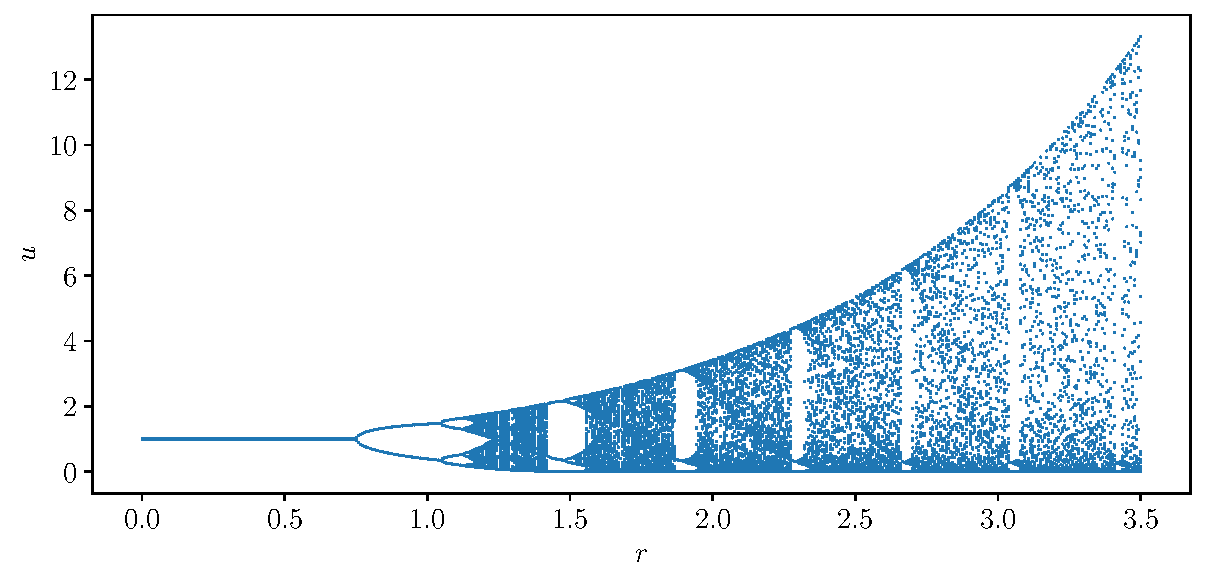
\includegraphics[width=\textwidth]{figures/bifurc1.pdf}
    \caption{Бифуркационная диаграма.}
    \label{fig:bifurc1}
\end{figure}

На графике видно, как неподвижная точка теряет устойчивость при $r=3\!/4$ и возникает цикл длины 2. 
Также видно, что существуют значения параметра, при которых для системы характерно хаотическое поведение.

\subsection{Показатель Ляпунова}

Показатель Ляпунова дискретной системы с правой частью $f(u)$ вычисляется следующим образом:
 \begin{equation}\label{eq:lyap}
     h(u) = \lim\limits_{n \rightarrow \infty}
     \frac{\ln \lvert f'(u_1) \rvert +\ldots + \ln \lvert f'(u_n) \rvert }{n}
.\end{equation} 
Данный показатель является мерой заотичности траекторий системы.
Если он меньше нуля, то близкие по начальным значениям траектории сходятся на бесконечности,
если меньше нуля, то близкие траектории сильно расходятся и система демонстрирует хаотическое поведение.
Для построения численной аппроксимации показателья Ляпунова было вычислено 1000 точек траектории для каждого значения параметра.
Получившийся график показан на рис.~\ref{fig:lyap}.

\begin{figure}[ht]
    \centering
    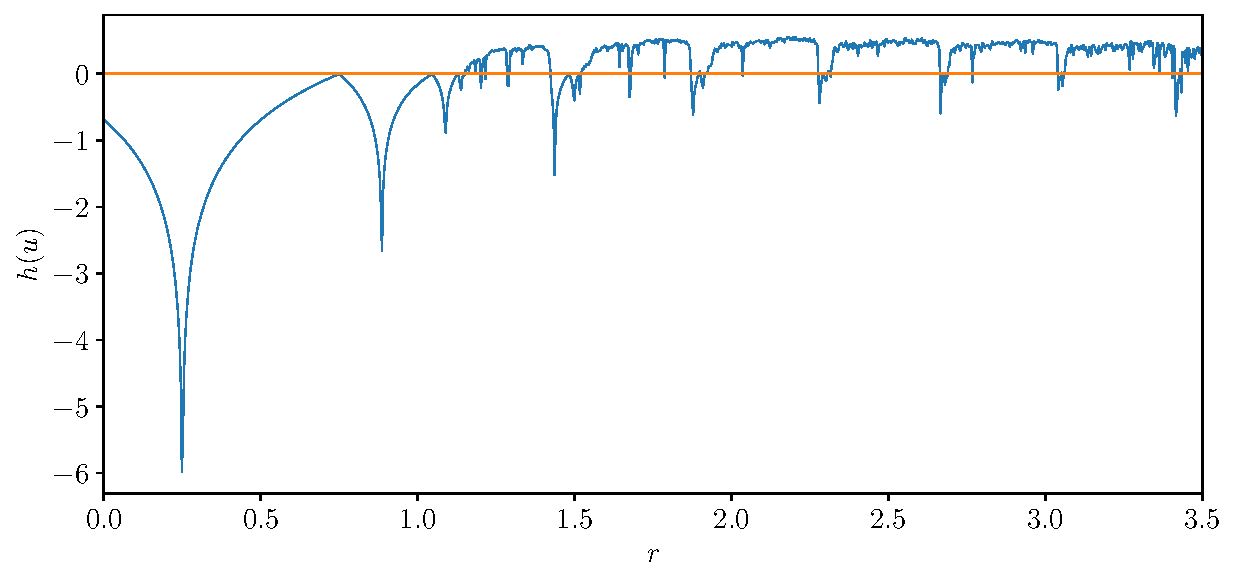
\includegraphics[width=\textwidth]{figures/lyap.pdf}
    \caption{Численная аппроксимация показателя Ляпунова.}
    \label{fig:lyap}
\end{figure}

Как видно из графика, существуют значения параметра $r$, при которых показатель Ляпунова положительный и система демонстрирует хаотическое поведени.
Моменты, когда показатель Ляпунова обнуляется, соответствуют точкам бифуркации системы.

\section{Двухшаговая система}

Перейдем теперь к исследованию системы с запаздыванием~\eqref{eq:2}.
Для этого положим $g(u, v) = \sqrt{u}\,e^{r(1-v^2)}$.
Здесь мы также полагаем параметр $b=1$, так как он не влияет на качественное поведение системы.
Тогда система с запаздыванием эквивалентна следующей двумерной системе:
 \begin{equation}\label{eq:2d}
    \begin{cases}
        u_{t+1} = g(u_t, v_t) = \sqrt{u_t}\,e^{r(1-v_t^2)},\\
        v_{t+1} = u_t.
    \end{cases} 
\end{equation} 

Заметим, что система~\eqref{eq:2} имеет те же неподвижные точки, что и одношаговая система, а именно: $u^*=0$ и  $u^*=1$.
Перейдем теперь к исследованию устойчивости неподвижных точек.

\subsection{Исследование устойчивости неподвжных точек}

Исследование тривиальной неподвижной точки $u^*=0$ проводится аналогично случаю без запаздывания. 
Точка будет неустойчивой.

Для исследования нетривиальной неподвижной точки выпишем матрицу Якоби системы~\eqref{eq:2d}:
\begin{equation}\label{Jac}
    J(u, v) = 
    \begin{pmatrix}
        \frac{e^{r(1-v^2)}}{2\sqrt{u}} & -2rv\sqrt{u}\,e^{r(1-v^2)} \\
        1 & 0
    \end{pmatrix} 
.\end{equation} 
В неподвижной точке $v^{*}=u^{*} = 1$ матрица Якоби принимает вид:
\begin{equation}\label{Jac_st}
    J(1, 1) = 
    \begin{pmatrix}
        1\!/2 & -2r \\
        1 & 0
    \end{pmatrix} 
.\end{equation} 
Для исследования устойчивости найдем собственный значения матрицы Якоби:
\begin{equation}\label{Jac_eig}
    \lambda_{1,2} = \frac{1 \pm \sqrt{1 - 32r}}{4}
.\end{equation} 

Далее рассмотрим отдельно действительный и комплексный случаи.
При $r \in (0, 1\!/32]$ оба собственных значения действительны и по модулю не превосходят единицы, поэтому будет асимптотическая устойчивость.

В при  $r > 1\!/32$ будет 2 комплексно-сопряженных собственных значения:
 \begin{equation}\label{eq:eig_compl}
     \lambda_{1,2} = \frac{1 \pm i\sqrt{32r - 1}}{4}, \quad 
     \lvert \lambda_{1,2} \rvert = \sqrt{2r}
.\end{equation} 
Таким образом, при $r < 1\!/2$ нетривиальная неподвижная точка будет асимптотически устойчивой, 
при $r > 1\!/2$"---~неустойчивой. 
Случай $r=1\!/2$ требует дополнительного исследования и рассматривается далее.

\bibliographystyle{utf8gost705u}
\bibliography{biblio}
 \end{document} 
